\documentclass[a4paper,10pt]{article}

\usepackage[margin=1in]{geometry} 	% Setea el margen manualmente, todos iguales.
\usepackage[spanish]{babel} 		% {Con estos dos anda
\usepackage[utf8]{inputenc} 		% todo lo que es tildes y ñ}
\usepackage{fancyhdr} 			%{Estos dos son para
\pagestyle{fancyplain} 			% el header copado}
\usepackage{color}			% Con esto puedo hacer la matufia de poner en color blanco un texto para engañar al formato
\usepackage{xcolor}
\usepackage{hyperref}
\usepackage{float}
\usepackage{framed}			%para crear cajas de texto
\usepackage{caratula}
\usepackage{verbatim}
\lhead{Teoría de las Comunicaciones}% {Con esto se usa el header copado. También está \chead para
\rhead{Trabajo Práctico Número 2} 	% el centro y comandos para el pie de página, buscar fancyhdr}


%%%%%%%%%%%%%%%%%%%%%%%%%%%%%%%%%%%%%
%      COMANDOS ÚTILES USADOS       %
%%%%%%%%%%%%%%%%%%%%%%%%%%%%%%%%%%%%%

% \section{title} 		Te hace un título ``importante'' en negrita, numerado. También está \subsection{title} y \subsubsection{title}.
% \begin{itemize}		Te hace viñetas.
%	\item esto es un item	Cambiar itemize por enumerate te hace una numeración.
% \end{itemize}

% \textbf{text} 		Te hace el texto en negrita (bold).
% \underline{text}		Te subraya el texto.

% \textsuperscript{text}	Te hace ``superindices'' con texto. En teoría subscript debería funcionar, pero se puede usar guion bajo entre llaves
% 				y signos peso para hacerlo como alternativa. Sino buscar.

% \begin{tabular}{cols} 	Es para hacer tablas. Se pone una c por cada columna deseada dentro de cols (si es que se desea centrada, l para justificar a 
%	a & b & c		izquierda, r a la derecha). Si se separa por espacios la tabla no tendrá líneas divisorias. Si se separa por | en lugar de 
% \end{tabular}			espacios, aparecerá una línea. Con || dos, y así. Luego para los elementos de las filas se escriben y se separan con ampersand (&).
%				Finalmente, para las líneas horizontales, se usa \hline para una linea en toda la tabla y \cline{i - j} te hace la linea desde
%				la celda i hasta la j, arrancando en 1.
%				Si en la columna se pone p(width) podés escribir un párrafo en la celda. Para hacer un enter con \\ no funciona porque te hace un
%				enter en la fila. Para eso se usa el comando \newline.
  
% \textcolor{color predefinido en palabras}{text}

%%%%%%%%%%%%%%%%%%%%%%%%%%%%%%%%%%%%%
%    FIN COMANDOS ÚTILES USADOS     %
%%%%%%%%%%%%%%%%%%%%%%%%%%%%%%%%%%%%%

\begin{document}

%%%%%%%%%%%%%%%%%%%%%%%%%%%%%%
%    Carátula										      %
%%%%%%%%%%%%%%%%%%%%%%%%%%%%%%



% parametros para la caratula (caratula.sty)


\materia{Teoría de las Comunicaciones}
\titulo{Trabajo Práctico 3}
\subtitulo{Capa de Transporte: Programación de protocolos end-to-end}
\fecha{14 de Noviembre de 2014}
\integrante{Juan Manuel Tastzian}{39/10}{jm@tast.com.ar}
\integrante{Lucas Tolchinsky}{591/07}{lucas.tolchinsky@gmail.com}
\integrante{Nicolás Vallejo}{500/10}{nico\_pr08@hotmail.com}

\maketitle

\newpage

%%%%%%%%%%%%%%%%%%%%%%%%%%%%%%%%%%%%
%    Tabla de contenidos/Índice    						%
%%%%%%%%%%%%%%%%%%%%%%%%%%%%%%%%%%%%

\setcounter{page}{1}

%-- Indice --
\newpage{\pagestyle{empty}\tableofcontents\cleardoublepage}

%%%%%%%%%%%%%%%%%%%%
%   Introducción    				 %
%%%%%%%%%%%%%%%%%%%%

\section{Introducción}

\subsection{Retransmission Timeout (RTO)}

El \textit{timeout de retransmisión} es un valor utilizado en protocolos como
\textbf{TCP} que sirve para \textit{asegurarse la entrega} de un paquete al
recipiente, a pesar de la ausencia de todo \textit{feedback} de su parte.\\
\\
\indent Para computar el \textbf{RTO} actual, el emisor del paquete mantiene dos
variables
de estado: \textbf{SRTT} (\textit{smoothed round-trip time}) y \textbf{RTTVAR}
(\textit{round-trip time variation}).\\
\\
\indent Cualquier implementación debe manejar el/los timer(s) de retransmisión
de forma tal que \textit{un segmento \textbf{nunca} es retransmitido demasiado
temprano} (es decir, en menos de un RTO luego de la transmisión del segmento
anterior).\\
\\
\indent A continuación, dejamos el algoritmo \textbf{recomendado} en el
\textbf{RFC 6298} para el manejo del timer de retransmisión:
\begin{enumerate}
 \item Cada vez que se envía un paquete con datos (incluyendo una
	retransmisión), si el timer no está corriendo, se inicia el mismo para
	que expire luego de \textit{RTO} segundos (para el valor actual de
	\textit{RTO}).
 \item Cuando se hizo \textit{ACK} de todos los datos, se apaga el timer de
	retransmisión.
 \item Cuando se recibe un \textit{ACK} que confirma nuevos datos, se reinicia
	el timer de retransmisión para que expire luego de \textit{RTO}
	segundos (para el valor actual de \textit{RTO}).
\end{enumerate}
Cuando expira el timer de retransmisión, hacer lo siguiente:
\begin{enumerate}
 \setcounter{enumi}{3}
 \item Retransmitir el segmento más viejo que no haya sido confirmado
	por el receptor de TCP.
 \item El emisor debe setear \textbf{RTO $\leftarrow$ RTO * 2} (``hacer
	\textit{back off} del timer"). Como valor para acotar superiormente
	esta operación, se puede usar el valor de 60 segundos.
 \item Comenzar el timer de retransmisión para que expire luego de \textit{RTO}
	segundos (para el valor de \textit{RTO} conseguido luego de hacer la
	operación de duplicación en el ítem número 5).
 \item Si expira el timer esperando el \textit{ACK} de un segmento \textit{SYN}
	y la implementación está usando un \textit{RTO} menor a 3 segundos, el
	\textit{RTO} debe ser re-inicializado a 3 segundos cuando comienza la
	transmisión de datos (es decir, luego de finalizar el three-way handshake).
\end{enumerate}

\newpage
\section{Desarrollo}

Para realizar las capturas de paquetes necesarias para la confección de este trabajo práctico se implementó una herramienta en python utilizando las bibliotecas de scapy.En el archivo \textit{sniffer.py} se encontrará el código fuente de la \textit{tool}. Consideramos oportuno mencionar que nuestra herramienta captura, en modo promiscuo, todos los paquetes que puede de la red local para luego volcarlo en un archivo con extensión \textit{.pcap}, soportado por aplicaciones como Wireshark.\newline

Si bien es cierto que scapy nos provee la funcionalidad suficiente como para simplemente capturar los ARP necesarios, nos pareció lógico que la herramienta capturase todo lo que pudiese, puesto que filtrar los datos con el Wireshark es bastante fácil de hacer.\newline

En el archivo \textit{helpers.py} se podrá encontrar todas las funciones encargadas del cálculo de las entropías de las fuentes origen y destino. Con ayuda de un intérprete de Python como \textit{iPython} dichas funciones son fácilmente aplicables.\newline

Sobre el cálculo de la entropía queríamos comentar ciertas cuestiones. En primer lugar, que en vez de la probabilidad de aparición de cada IP utilizaremos la frecuencia de aparición de dicha dirección como fuente o destino de toda la captura dependiendo del caso. En segundo lugar, que calculamos para cada caso la frecuencia de aparición de todas las IP's tanto origenes como destino y luego realizamos el cálculo de la entropía. Notar que si una IP sólo aparece como fuente no impactará en el cálculo de la entropía para la fuente de IP's destino y viceversa, puesto que su frecuencia de aparición en dicha fuentes será igual a cero.\newline

Además, se implementaron dos scripts en Python que se encargan de, dado un archivo .pcap, exportar a formatos .tgf (Trivial Graph Format) y .dot respectivamente, que nos ayudaran para la armado de los grafos.\newline

Como hemos mencionado anteriormente, nuestro capturador no captura únicamente paquetes ARP who-has. Para obtener solamente esos paquetes, al archivo .pcap exportado por el script lo filtramos con la guarda \textit {arp.opcode= = 1 \&\&  !arp.isgratuitous} con Wireshark y luego lo exportamos a otro archivo .pcap que sólo contendrá los paquetes ARP who-has no gratuitos (los paquetes gratuitos son aquellos que algún host envía con su dirección para que los demás host de la red puedan actualizar su tabla de direcciones).\newline

\newpage
\section{Análisis}

El primer experimento que creímos útil es la prueba de suficientes combinaciones significativas de valores de $\alpha$ y $\beta$ para intentar identificar un par de valores de óptimo comportamiento. Esto lo hicimos fijando otras variables en algunos valores que nos parecieron coherentes (delay de 2 segundos y sin indeterminismo en los dropeos), para sólamente mirar dichas variables.\\

\indent Para poder evaluar esto, elegimos valores entre 0.1 y 0.9, aumentando en cada paso en 0.1 la variable analizada. Probamos algunos valores en el medio pero consideramos que aumentar la granularidad no nos daría cambios significativos en los resultados. Esto nos da una matríz de 81 resultados, los cuales, para poder analizarlos, partimos en 9 gráficos\footnote{Aparte de estas imágenes, debajo de cada uno se encuentra un link a su versión interactiva, para poder apreciar mejor los datos.}, fijando cada valor de $\alpha$ y graficando las variaciones de los $\beta$.\\

\indent En todos los gráficos, aparte del resultado de cada $\beta$ con el $\alpha$ de dicha corrida, se encuentra una línea constante que representa el \textbf{promedio de RTT} el cual en el caso ideal, sería el mismo valor que el \textbf{RTO}. La elección de mejor par de $\alpha$ y $\beta$ la hicimos bajo este criterio, viendo para cada valor de $\alpha$, el valor de $\beta$ que más rápido llega a parecerse al RTT promedio y el que más estable se mantiene a lo largo de las pruebas (pues puede que alguno llegue rápido pero luego de algunas iteraciones empiece a mostrar comportamiento errático y no sea tan bueno en general).

\begin{center}
	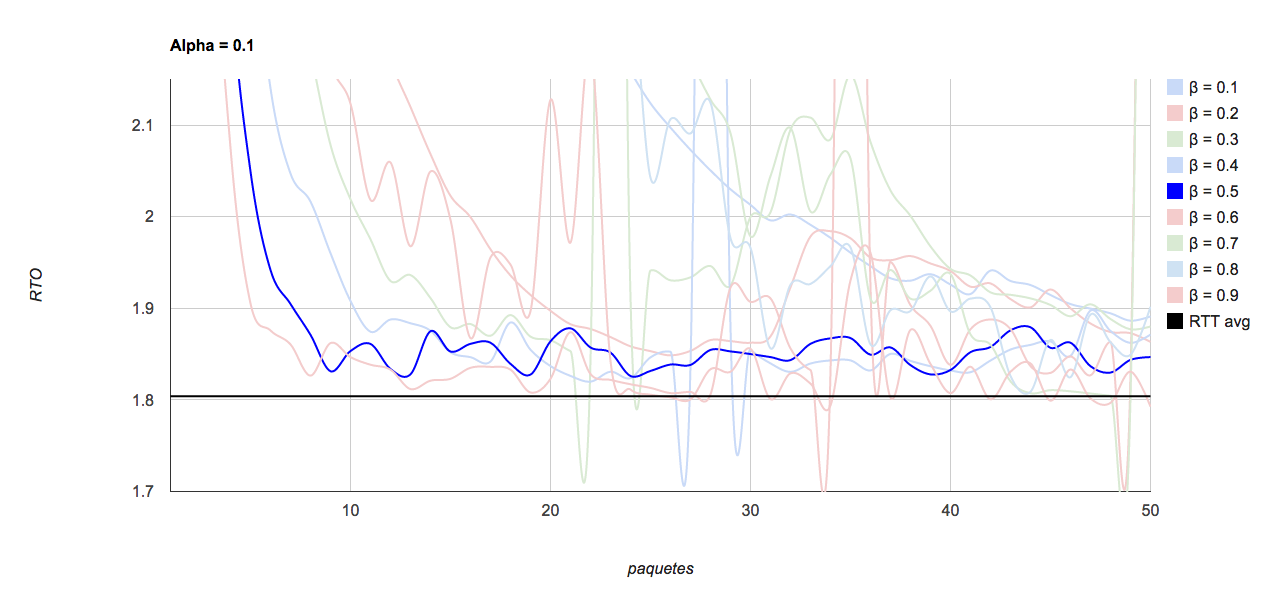
\includegraphics[scale=0.35]{graphics/rto_vs_paquetes_a_1.png}
	\textit{Gráfico interactivo en:} http://goo.gl/i3q8vd
\end{center}

\begin{center}
	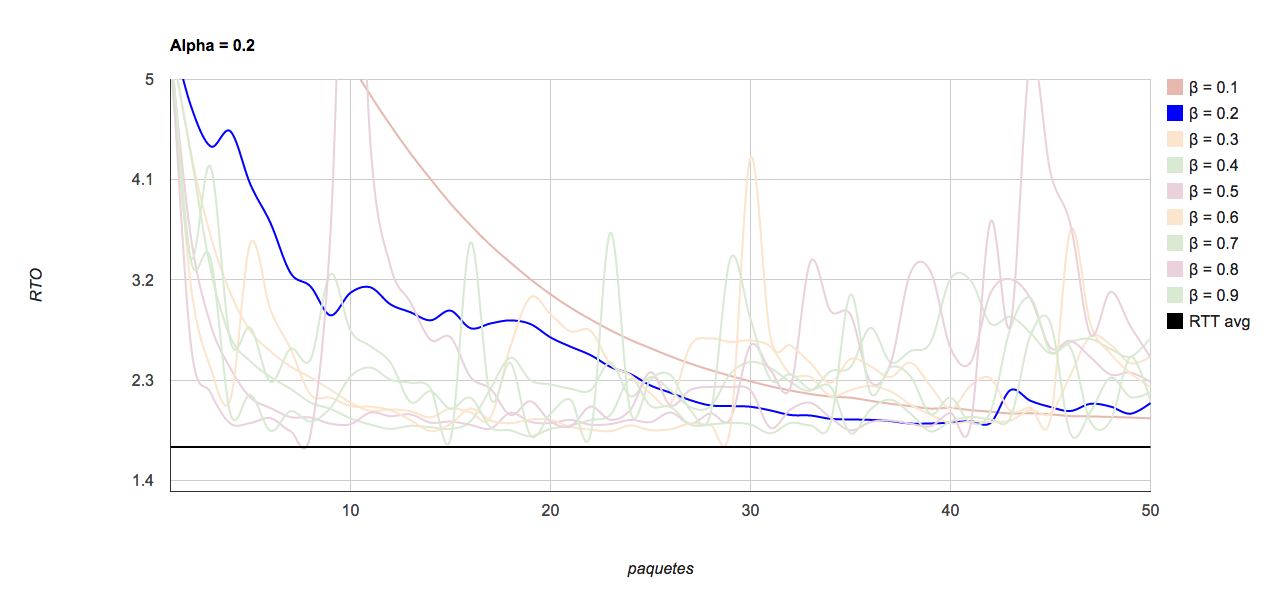
\includegraphics[scale=0.35]{graphics/rto_vs_paquetes_a_2.png}
	\textit{Gráfico interactivo en:} http://goo.gl/QS0NjO
\end{center}

\begin{center}
	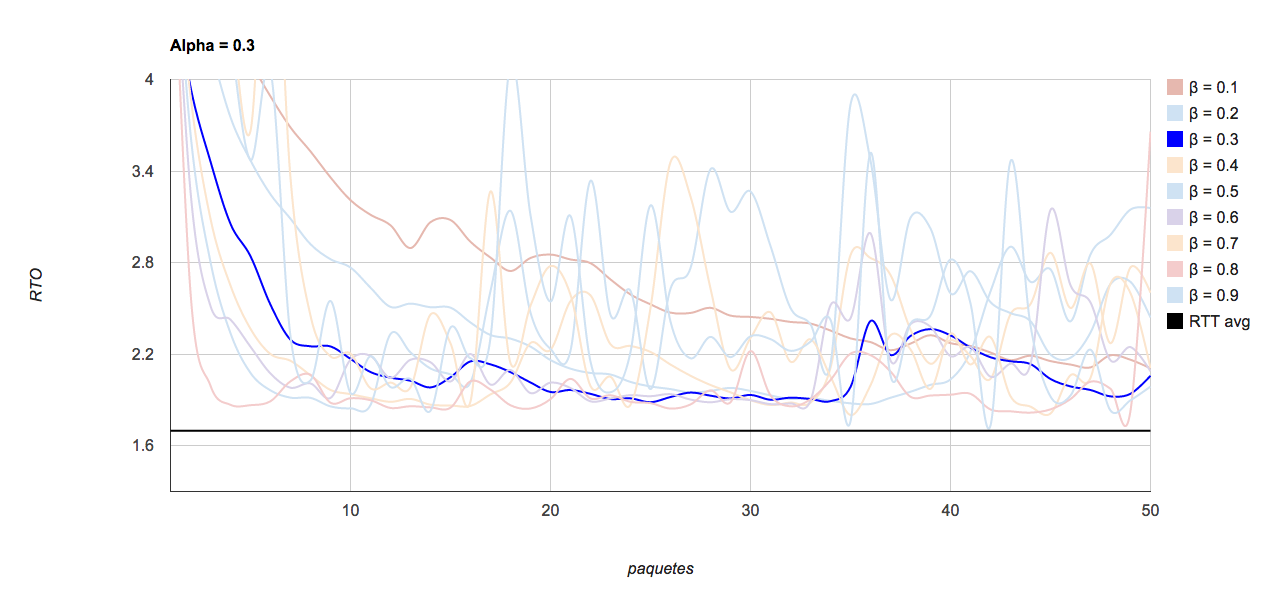
\includegraphics[scale=0.35]{graphics/rto_vs_paquetes_a_3.png}
	\textit{Gráfico interactivo en:} http://goo.gl/cmSyGd
\end{center}

\begin{center}
	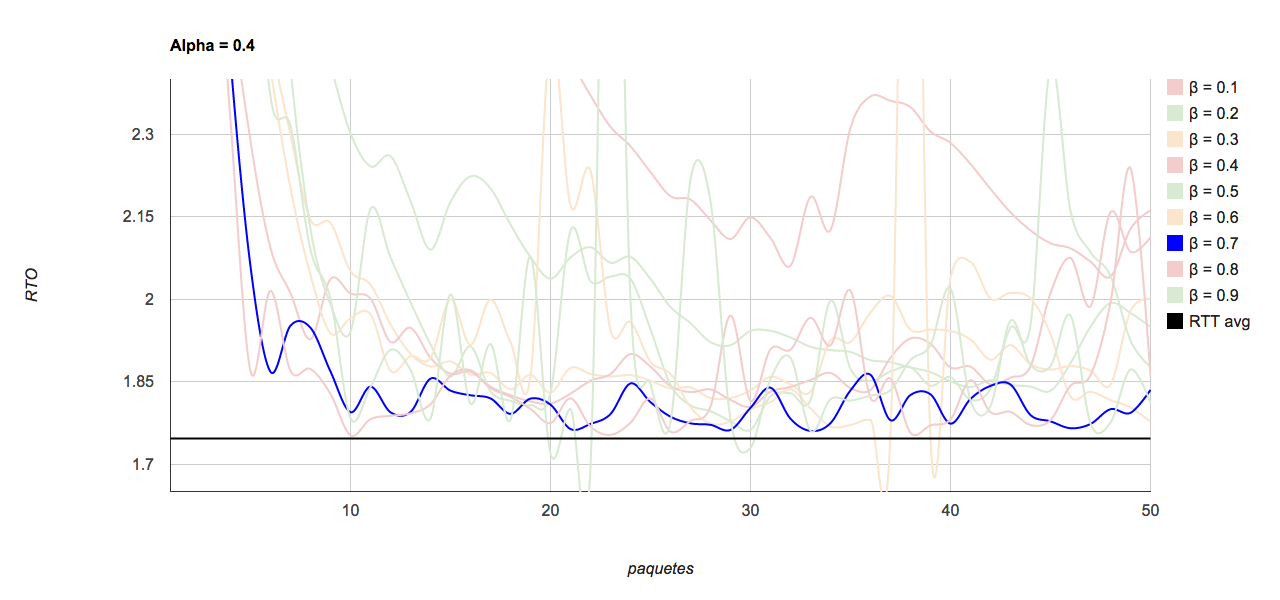
\includegraphics[scale=0.35]{graphics/rto_vs_paquetes_a_4.png}
	\textit{Gráfico interactivo en:} http://goo.gl/Db08yU
\end{center}

\begin{center}
	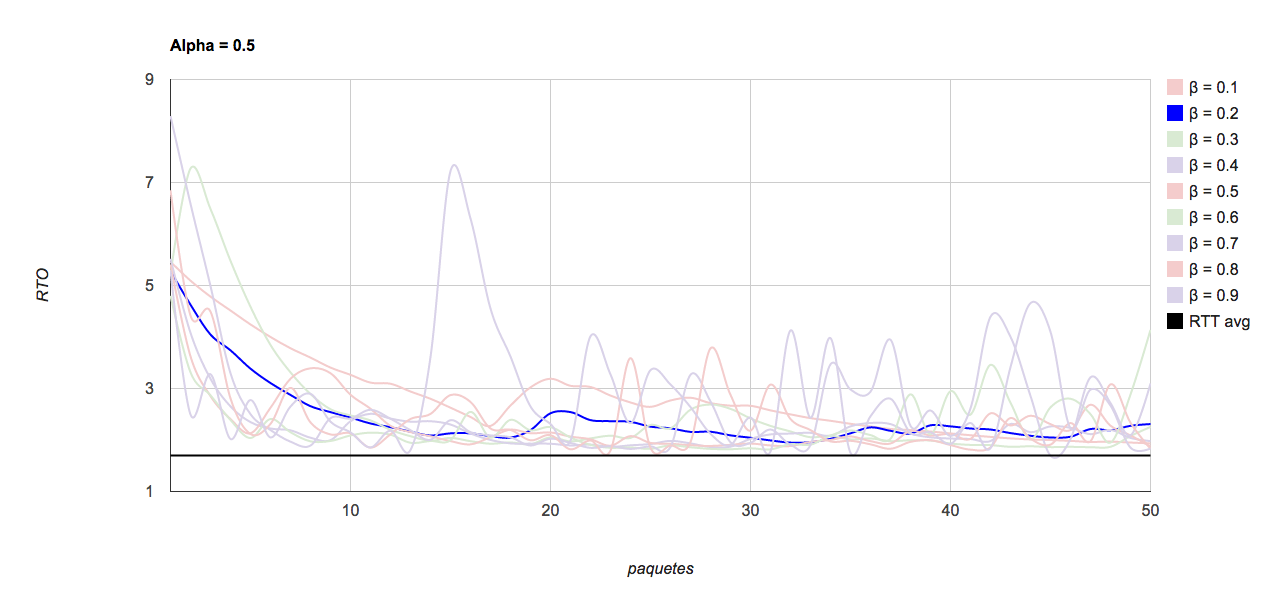
\includegraphics[scale=0.35]{graphics/rto_vs_paquetes_a_5.png}
	\textit{Gráfico interactivo en:} http://goo.gl/VNV8xF
\end{center}

\begin{center}
	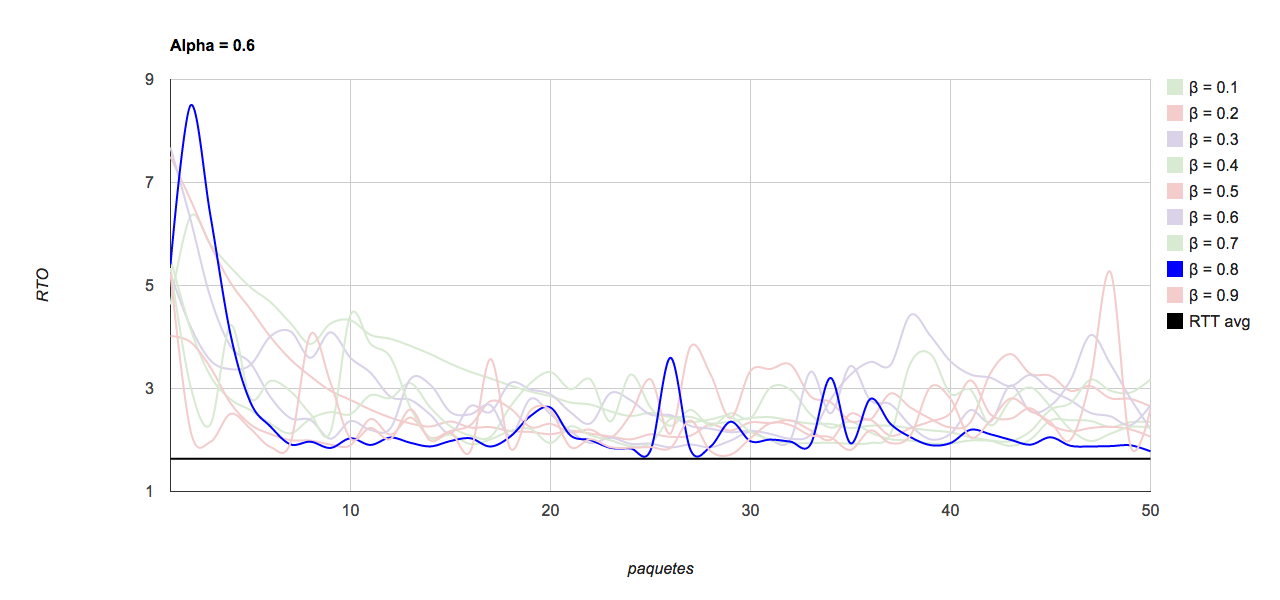
\includegraphics[scale=0.35]{graphics/rto_vs_paquetes_a_6.png}
	\textit{Gráfico interactivo en:} http://goo.gl/CN4joc
\end{center}

\begin{center}
	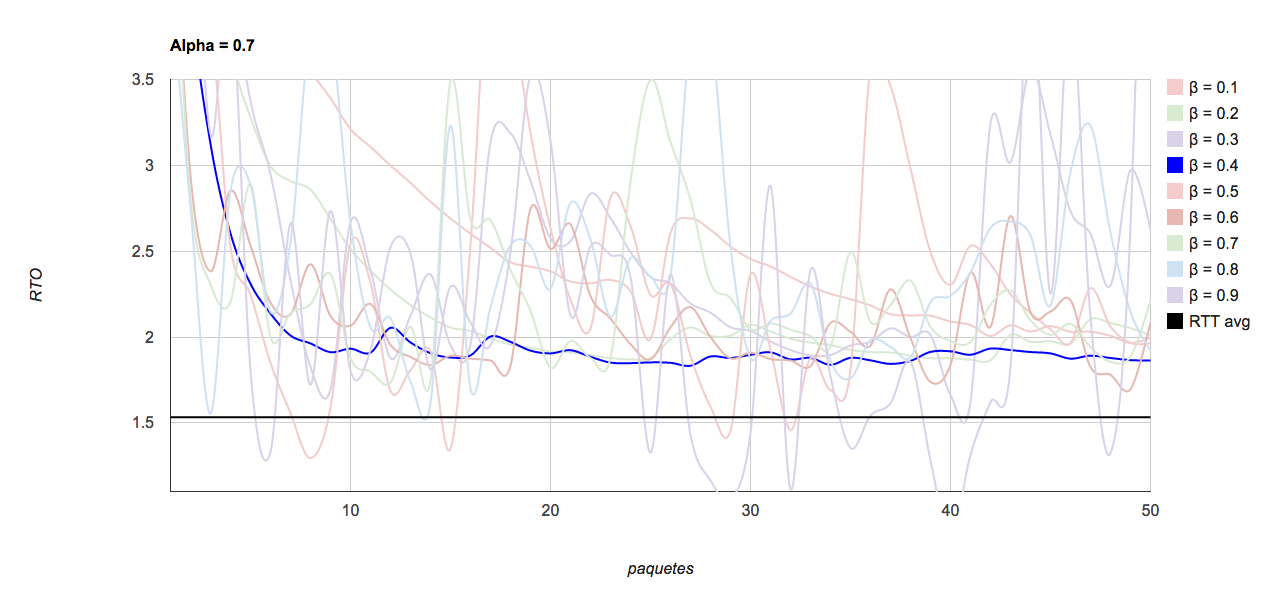
\includegraphics[scale=0.35]{graphics/rto_vs_paquetes_a_7.png}
	\textit{Gráfico interactivo en:} http://goo.gl/Gc93dU
\end{center}

\begin{center}
	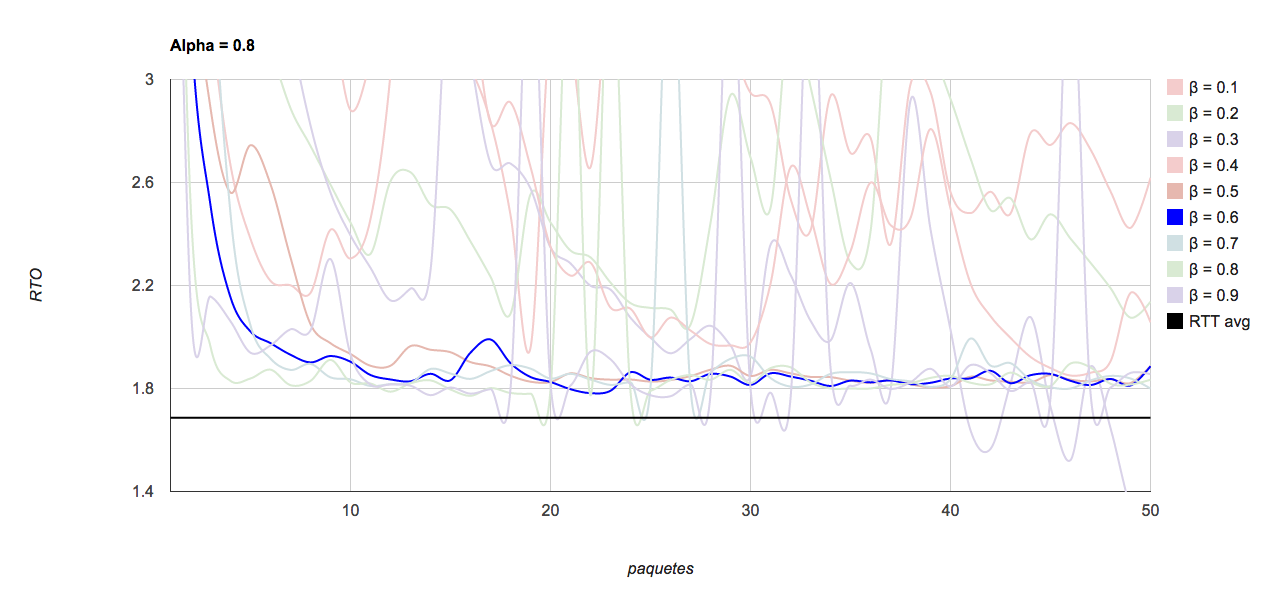
\includegraphics[scale=0.35]{graphics/rto_vs_paquetes_a_8.png}
	\textit{Gráfico interactivo en:} http://goo.gl/RGiQc0
\end{center}

\begin{center}
	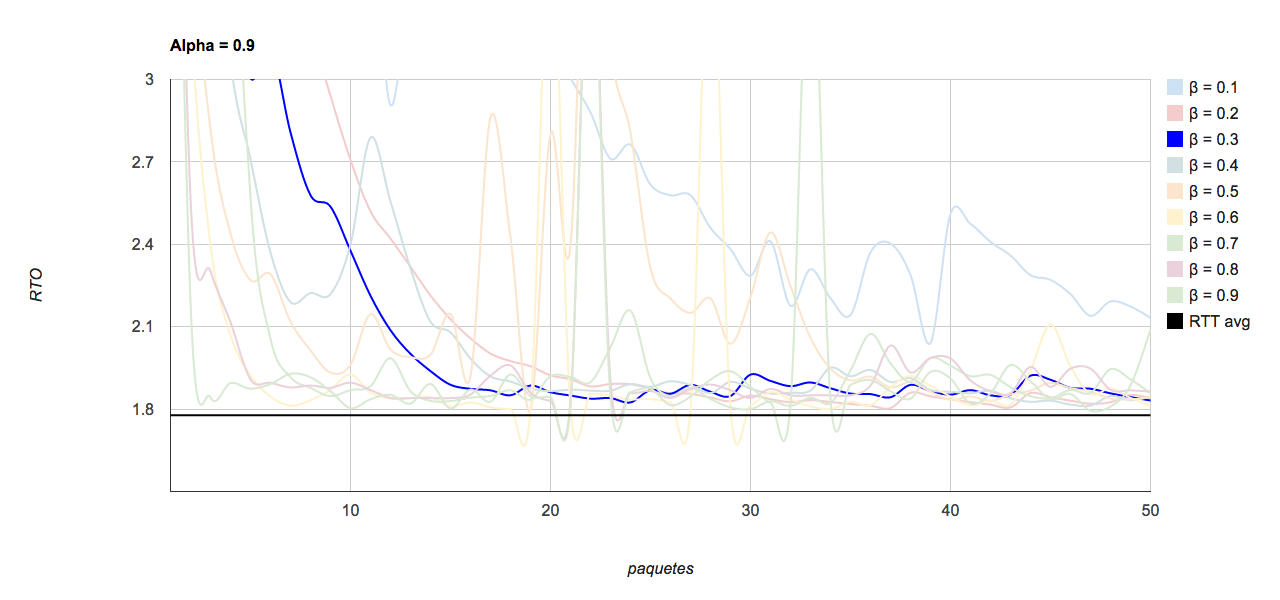
\includegraphics[scale=0.35]{graphics/rto_vs_paquetes_a_9.png}
	\textit{Gráfico interactivo en:} http://goo.gl/QXH7cA
\end{center}

De cada uno de los gráficos, extrajimos el mejor par $\alpha$, $\beta$ y los juntamos en un mismo gráfico para, entre ellos, elegir el mejor de las 81 posibilidades. Según esta experimentación, entonces, los mejores valores en este protocolo para $\alpha$ y $\beta$ en nuestro caso, nos dieron cuando $\alpha = 0.4$ y $\beta = 0.7$.

\begin{center}
	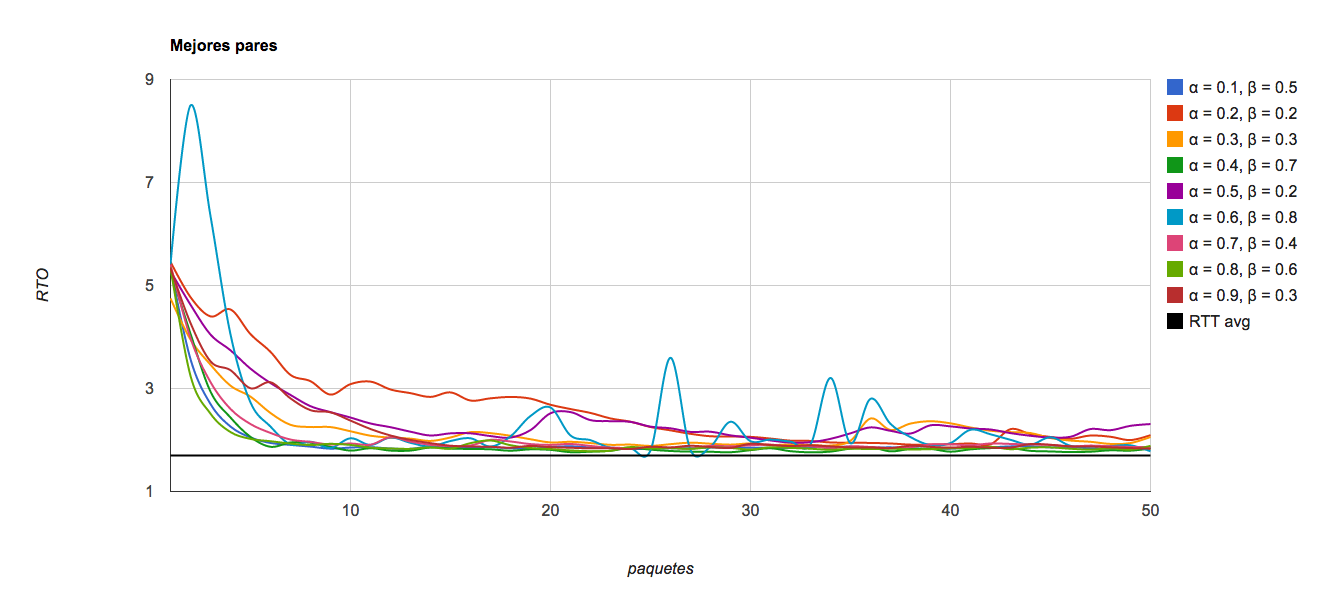
\includegraphics[scale=0.35]{graphics/best_pairs.png}
	\textit{Gráfico interactivo en:} http://goo.gl/FBA1p2
\end{center}

El gráfico anterior lo dejamos para dimensionar la convergencia y los valores en general. El siguiente gráfico es el que realmente hace notar que de todas las opciones, la anteriormente elegida es la que más cerca se encuentra del promedio de RTT, y además, la que más estable mantiene dicha cercanía.

\begin{center}
	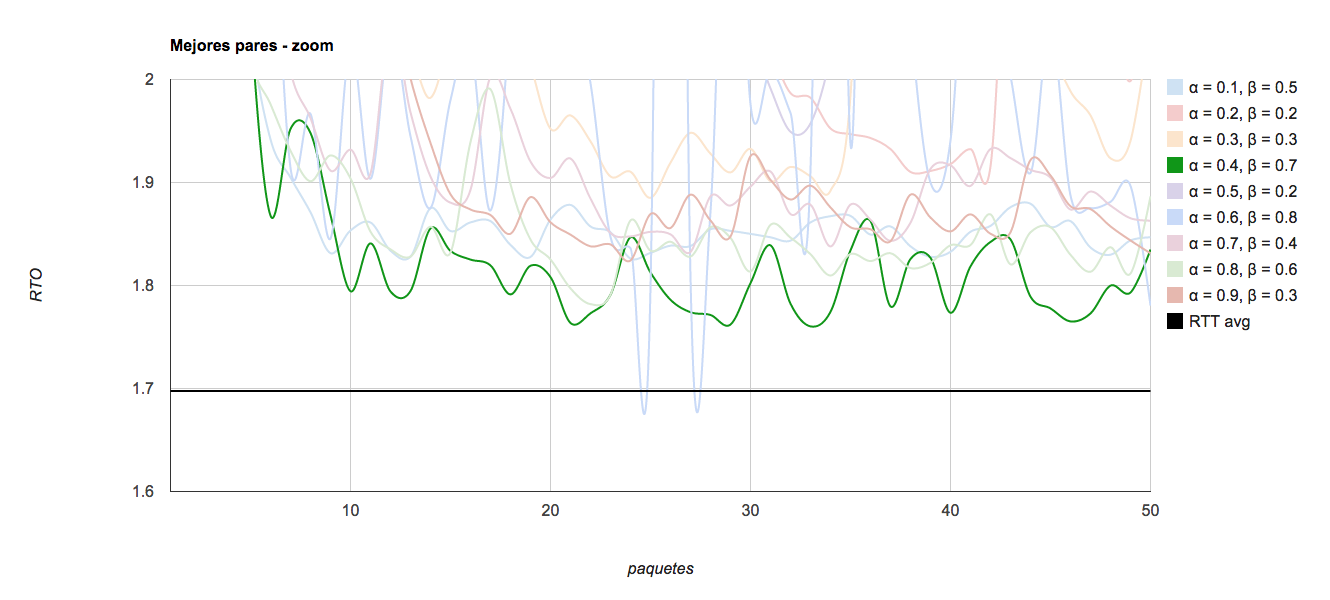
\includegraphics[scale=0.35]{graphics/best_pairs_zoom.png}
	\textit{Gráfico interactivo en:} http://goo.gl/RvuVpr
\end{center}

%\input{biblio.tex}
\newpage











%%%%%%%%%%%%%%%%%%%%%%%%%%%%%%%%%%%%%%%%
%        Esto es de mi template        %
%    Dejar para futuras referencias    %
%%%%%%%%%%%%%%%%%%%%%%%%%%%%%%%%%%%%%%%%

% \section{Sección, título grande}
% \\
% \textcolor{white}{Sarasa engañadora de formato, jua jua}\\
% Esto es texto. Con doble barra invertida es el enter.
% \\
% \\
% \textit{De acá en adelante, todo lo que se explica como "para hacer x se usa y", implica que antes de y va una barra invertida}
% \\
% \\
% Con \textbf{textbf\{\}} se escribe en negrita.
% \\
% \\
% \section{Bullet \& Numbering}
% Para hacer items se usa \textbf{begin\{itemize\}} y \textbf{end\{itemize\}}, por ejemplo:
% \begin{itemize}
% 	\item Esto es un ítem.
% 	\item Esto es otro.
% \end{itemize}
% Con \textbf{item} se hace cada uno de los ítems. Si cambiás \textbf{itemize} por \textbf{enumerate} te lo hace enumerado. Por ejemplo:
% \begin{enumerate}
% 	\item Acá está el primero.
% 	\item Acá el segundo.
% \end{enumerate}
% \\
% Y así.
% \\
% \\
% \section{Tablas}
% También tenemos las tablas, que son un poco más rebuscadas. Se usa \textbf{begin\{tabular\}\{cols\}} y en cols ponemos c si queremos una columna centrada, l y r
% para otro tipo de justificación. Si las c las separás con espacios, se hacen columnas sin división. Si ponés un pipe es con una línea divisoria, dos pipes con
% dos líneas, y así. Se termina con \textbf{end\{tabular\}}. Para separar entre elementos de fila/columna se usa un ampersand (\&, y es necesario para separar
% elementos entre filas y columnas, no solo entre filas) y para cambiar de fila \textbf{SIN} linea divisoria, un \textbf{newline} ya que el doble barra invertida
% te hace un enter dentro de la celda. Con línea divisoria es reemplazando \textbf{newline} por \textbf{hline}.
% \\
% \\
% Más datos en el principio de este tex. Un ejemplo:
% \\
% \\
% \begin{tabular}{| c| c|}\hline
%     Celda 1 & Celda 2 &\hline
%     Celda 3 & Celda 4 &\hline
% \end{tabular}
% \\
% \\
% \section{Verbatim}
% \begin{verbatim}
% Esto es verbatim. Es un entorno que no le da ni 5 de pelota al formato de latex.
% Por eso mismo hay que tener cuidado con no irse de la hoja o similar.
% Sirve por ejemplo, para pseudocódigo:
% 
% if (se cumple sarasa){
%     ejecuto cosito1;
%     ejecuto cosito2:
% }else{
%     ejecuto cosito3:
% }
% \end{verbatim}

\end{document}
